\documentclass[a4paper,12pt]{report}
\usepackage[left=2cm,right=2cm,top=2cm,bottom=2cm]{geometry}
\usepackage[T1]{fontenc}
\usepackage[utf8]{inputenc}
\usepackage{ngerman}
\usepackage{amsmath}
\usepackage{charter}
\usepackage{graphicx}
\usepackage{tikz}

\begin{document}
	\noindent
	\Large
	1.9.3 Kombiniere 1.9.1 mit 1.9.2: Der elektrische Schwingkreis
	\hrule
	\large
	\vspace{1cm}
	\noindent
	BILD \\
	Situationen (temporär): \\
	1)
	BILD
	\\
	t = 0 \\\\
	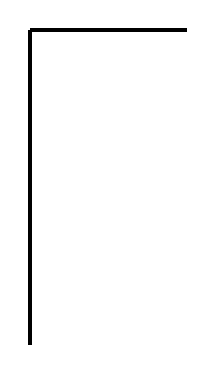
\begin{tikzpicture}
		\draw [ultra thick] (2,0) -- (2,4);
		\draw [ultra thick] (2,4) -- (4,4);
	\end{tikzpicture}
\end{document}